\documentclass{article}
\usepackage[utf8]{inputenc}
\usepackage{graphicx}
\graphicspath{/Users/nikourriola/Desktop/Spring 2019/phys403/muon lab/}

\title{Muon lifetime data system calibration and capture electronics configuration}
%\title{Muon Lifetime Data Acquisition Configuration}

\author{Vishnu Chavva and Elliot Urriola }
\date{February 6, 2019}

\begin{document}

\maketitle

%Abstract section
\begin{center}
    %abstract should be centered
    \section*{Abstract}
    Hello world.  
\end{center}

%Introduction section
\section*{Introduction}

\hspace{3.5mm} Supernovae located well outside the Earth's solar system often emit high-energy radiation called cosmic rays. These cosmic rays are mostly comprised of protons [1]. %[cosmic ray muons slides]
Eventually, the cosmic rays reach Earth's  upper atmosphere, where the constituent protons most frequently collide with diatomic molecules [1]. %[cosmic ray muons slides]
This interaction begins a series of decay processes which produce an array of new particles. Among these product particles are muons. Muons are charged, fundamental fermions that are related to electrons. Cosmic rays serve as the most abundant source of muons on earth, providing approximately 1 muon per square centimeter every minute at sea level.   

Current areas of research involving the muon often require complicated collider systems and sophisticated electronics. Additionally, progressing this technology has become an important part of physics research beyond the standard model [2]. %[collider]
However, much simpler experiments have been designed to exemplify the research concepts used in high energy physics [3]. %[undergrad]

%These simplified experiments focus on a determination of the muon lifetime. The readout electronics are much simpler than the electronics built for collider experiments, and often use scintillators attached to photomultiplier tubes (PMT) as a detection mechanism [0]. %[undergrad] 


Specifically, simplified experiments focus on a determination of muon lifetime in order to investigate weak interaction phenomena. Muon decay is a process driven entirely by the weak force [4]. %[gfriffiths pcl physics]
So, it is possible to measure the strength of the weak force by measuring muon lifetime. This relationship is summarized by Equation 1 where $\tau_{\mu}$ is muon lifetime and \textit{G$_{F}$} is a constant called the Fermi Coupling Constant. A rigorous derivation of Equation 1 is found in Griffiths chapter 9.2 [4]. %[Griffiths]   

%Equation 1
\begin{center}
    
    $\tau_{\mu} = \frac{192 \pi^3}{\textit{G$_{F}$}^2 m_{\mu}^5}$ \hspace{10mm} \textbf{(1)}
    
    \vspace{5mm}
    
    \textbf{Equation 1.} Muon lifetime is proportional to the inverse square of the Fermi Coupling Constant.
    
\end{center}


\textit{G$_{F}$} is the quantity that describes the strength of the weak force. As such, \textit{G$_{F}$} is necessary for all calculations of weak interaction phenomena [5]. %[3 constants] 
Thus, a precise value for \textit{G$_{F}$} improves the accuracy of such calculations.

The main goal of this experiment is to calculate \textit{G$_{F}$} from a measurement of muon lifetime. We follow a procedure similar to the simplified procedure [3] %undergrad
described above to record muon decay events over several days. The electronics configuration and data acquisition will be used in further muon investigation experiments. 

From Equation 1, it is clear that determining \textit{G$_{F}$} could be achieved by a measurement of muon lifetime. The lifetime of a muon can be thought of as the inverse of the muon disappearance rate $\Gamma_{diss.}$. This relationship is shown in Equation 2. 

%Equation 2
\begin{center}

    %dissapearance rate and muon lifetime relationship
    %$\tau_{\mu} = \frac{1}{\Gamma_{diss.}}$ \hspace{10mm} \textbf{(2)}
    $\Gamma_{diss.} = \frac{1}{\tau_{\mu}}$ \hspace{10mm} \textbf{(2)}
    
    \vspace{5mm}
    
    \textbf{Equation 2.} Muon lifetime is the inverse of disappearance rate
    
\end{center}

A muon can dissappear by decaying according to the process shown in Equation 3. These decay processes are different depending on the charge of the muon at the time of decay. 

%Equation 3
\begin{center}
    
    %positive muon decay
    $\mu^{+} \rightarrow e^{+} + \nu_{e} + \overline{\nu}_{\mu}$ \hspace{10mm} \textbf{(3.a)}
    
    \vspace{1 mm}
    
    %negative muon decay; symmetric
    $\mu^{-} \rightarrow e^{-} + \overline{\nu}_{e} + \nu_{\mu}$ \hspace{10mm} \textbf{(3.b)}
    
    \vspace{5mm}
    
    \textbf{Equation 3.} Muon decay equations for \textbf{a)} positively charged muons. \textbf{b)} negatively charged muons 
    
\end{center}
  
However, negatively charged muons do not always decay. Some may interact with protons from the incoming cosmic rays and disappear according to Equation 4. 

%Equation 4
\begin{center}
    
    %negative muon decay; symmetric
    $\mu^{-} + \textit{p} \rightarrow \textit{n} +  \nu_{\mu}$ \hspace{10mm} \textbf{(4)}
    
    \vspace{5mm}
    
    \textbf{Equation 4.} Alternative disappearance process for negatively charged muons 
    
\end{center}

Thus, an expansion of Equation 2 holds for negatively charged muons. The expansion is seen in Equation 5. 
%Equation 5
\begin{center}
    
    %expansion of muon disappearance rate
    $\Gamma_{diss._{\mu^{-}}} = \Gamma_{decay} + \Gamma_{interact}$ \hspace{10mm} \textbf{(5)}
    
    \vspace{5mm}
    
    \textbf{Equation 5.} Expansion of Equation 2 for negatively charged muons
    
\end{center}

The additional disappearnce mode for negatively charged muons further complicates the muon lifetime measurement. That is, while the detection electronics in these simplified experiments are sensitive to the energy deposited by the muon decay products (Equation 3), they are unable to discern exactly how the muon disappeared. Adjustments are made when calculating the muon lifetime based on data acquired during the experiment and prior knowledge of cosmic ray composition [1]. %[cosmic ray composition] 

%Procedure Section
\section*{Procedure}
\hspace{3.5mm} Much of the experimental set up was already assembled before taking ownership. Specifically, the scintillator configuration shown in Figure 1 was already constructed.  

%Figure 1
\begin{center}

    \vspace{5mm}
    
    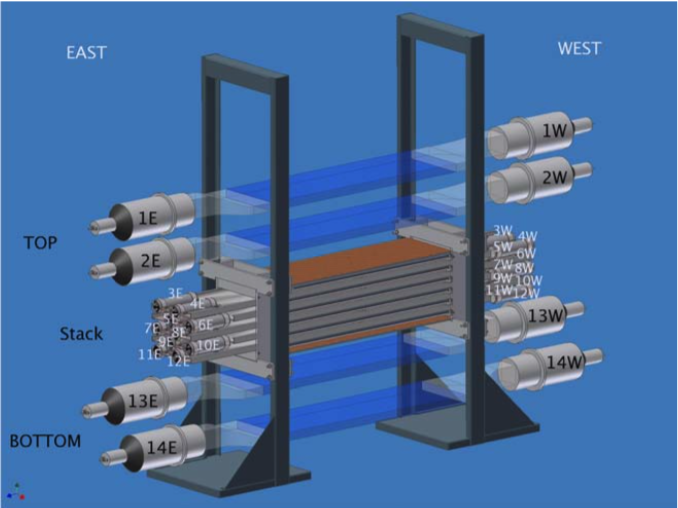
\includegraphics[width = \textwidth]{Figure1.png}   
    
    \vspace{5mm}
    
    \textbf{Figure 1.} Scintillator and photomultiplier tube (PMT) configuration
    
\end{center}

It is reccomended that the integrity of the top and bottom paddles be checked using a flashlight and ammeter. Namely, shining a flashlight over the surface of the scintillator and using the ammeter to measure the photomultiplier tube (PMT) output current. This preliminary check is one way to coarsely determine if there are any faults with the scintillator material or PMTs before calibration. However, this check was not done during our run of the experiment. 

The trigger electronics were built according to the circuit diagram shown in Figure 2. Models numbers for only select discriminators, time to digital converters (TDC), and logic units are given. These models can also be seen in Figure 2. The remaining logic and electronics are provided using standard nuclear instrumentation module (NIM) units.

%Figure 2
\begin{center}

    \vspace{5mm}
    
    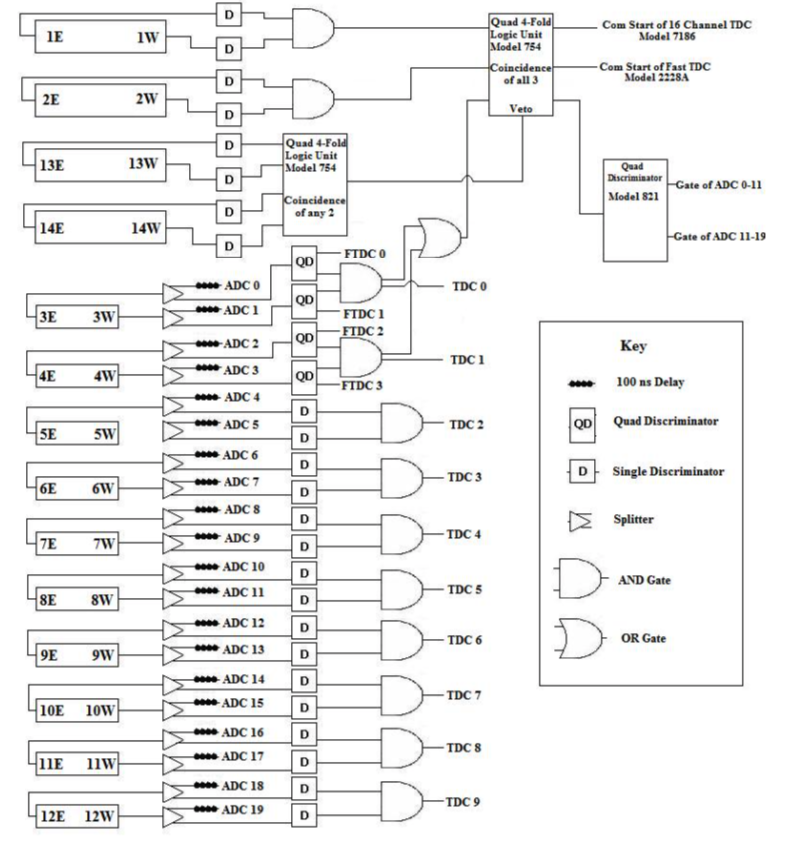
\includegraphics[width = \textwidth]{Figure2.png}

    
    \vspace{5mm}

\end{center}

In accordance with the layout in Figure 2, the start trigger electronics were built first. That is, the PMTs connected on either end of scintillator 1 and scintillator 2 were sent to single discriminators before entering logic AND gates. The discriminators provide a way of clearing up noise surrounding the event signal by outputting precise logic pulses based on the input signal. This output signal is responsible for starting the timer built into the electronics system. 

The pass through scintillators (BOTTOM in Figure 1) were connected much in the same way. The output of these single discriminators were used as inputs to a Quad 4-Fold Logic Unit according to Figure 2. Registering an event at these scintillators would indicate a muon passed through the target decay region of the stack. The downstream connection to the veto of a second Quad 4-Fold Logic Unit could be used to translate this information as a timeout for the TDC units. In turn, the data acquisition system can ignore this particular event.

Next, the stack was wired according to Figure 2. The PMT outputs of the stack were split prior to taking ownership of the experiment. So, one part of the split signal was delayed by 100 ns before being input to a 24 channel analog to digital converter (ADC) unit. The other part of the split signal was fed into either a single or quad discriminator, again, according to Figure 2. 

Each quad discriminator was connected to a fast time to digitial converter (FTDC). Although not shown in Figure 2, these connections were delayed by 100 ns before going into the FTDCs. This delay was manually added to ensure that the stop signal electronics did not fire before the start signal initiates the timer. Doing so would cause the TDC to timeout for all events because the command order would be reversed. The exact length of this delay was chosen based only on the availability of connections on the variable delay and 100 ns delay racks. A longer delay might be used, but some testing with known signals would be necessary.



%Results Section 
\section*{Results}

%Discussion Section
\section*{Discussion}

%Conclusions Section
\section*{Conclusion}

%References Section
\section*{References}

\hspace{4mm} [1] \hspace{1mm}  Anthony Tatum, "Cosmic Ray Muons," \textbf{https://uncw.edu/phy}\newline (February 1, 2019)

\vspace{3mm}

[2] \hspace{1mm} M. S. Zisman, Lawrence Berkeley National Laboratory (2011)

\vspace{3 mm}



[3] \hspace{1mm}  D. Bosnar, et. al, A simple setup for cosmic muon lifetime measurements, \textit{Eur. J. Phys.} \textbf{39}, 4 (2018)
\vspace{3 mm}

[4] \hspace{1mm} D. Griffiths, "Decay of the Muon," in \textit{Introduction to Elementary Particles}, Wiley-VCH; 2nd edition, Ch. 9, pp. 310 - 315

\vspace{3 mm}

[5] \hspace{1mm} T. van Ritbergen and R. G. Stuart, Complete 2-loop quantum electrodynamic contributions to the muon lifetime in the fermi model, \textit{Phys. Rev. Lett.} \textbf{82}, 488 (1999).























\end{document}
